(This this the start page of the LND GCR and albedo protons)


The moon is expose to the deep space. 


GCE from outside of Solar system, accelerated by the shock wave.


From 2019.1 to 2020.7, apart from the SEP event that we studied in the last chapter, no SEPs arrived on the lunar surface during this period, 
hence it is a good opportunity to study the galactic cosmic rays (GCRs) and the albedo protons.




GCR dominate the quite time
LND start from solar minimum, good opptunity to study the GCR

Beside,


We reproduced the following article from the published paper \citep{xu2020} under the CC BY 4.0 license as following and in the end of this , we give the configuration changes since LND landed and launched. 

The following articles is reproduced from the published paper \citep{xu2022} under the CC BY 4.0 license.






The following article is reproduced from \textcite{Xu-2022-LND-GCRalbedo}, which is an open-access article reproducted under the terms of 
the CC-BY license. The supplement material including the configuration changes of LND up to now and the data we used in the main content is attached afterward. 
\\

\noindent\pubcite{Xu-2022-LND-GCRalbedo}\\
\strut\hfill Own contribution: 90\%

\newpage
\newcounter{includepdfpageFrontierTwentyTwo}

\addtocounter{subsection}{1}
\setcounter{subsubsection}{1} 
\phantomsection
\addcontentsline{toc}{subsection}{\arabic{chapter}.\arabic{section}.\arabic{subsection} Primary and albedo protons detected by the Lunar Lander Neutron and Dosimetry experiment on the lunar farside(Publication Frontier in Astronomy and Space Sciences 2022)}
%
\phantomsection
\addcontentsline{toc}{subsubsection}{\arabic{chapter}.\arabic{section}.\arabic{subsection}.\arabic{subsubsection} Introduction}
\label{sec:paper_xu2022}
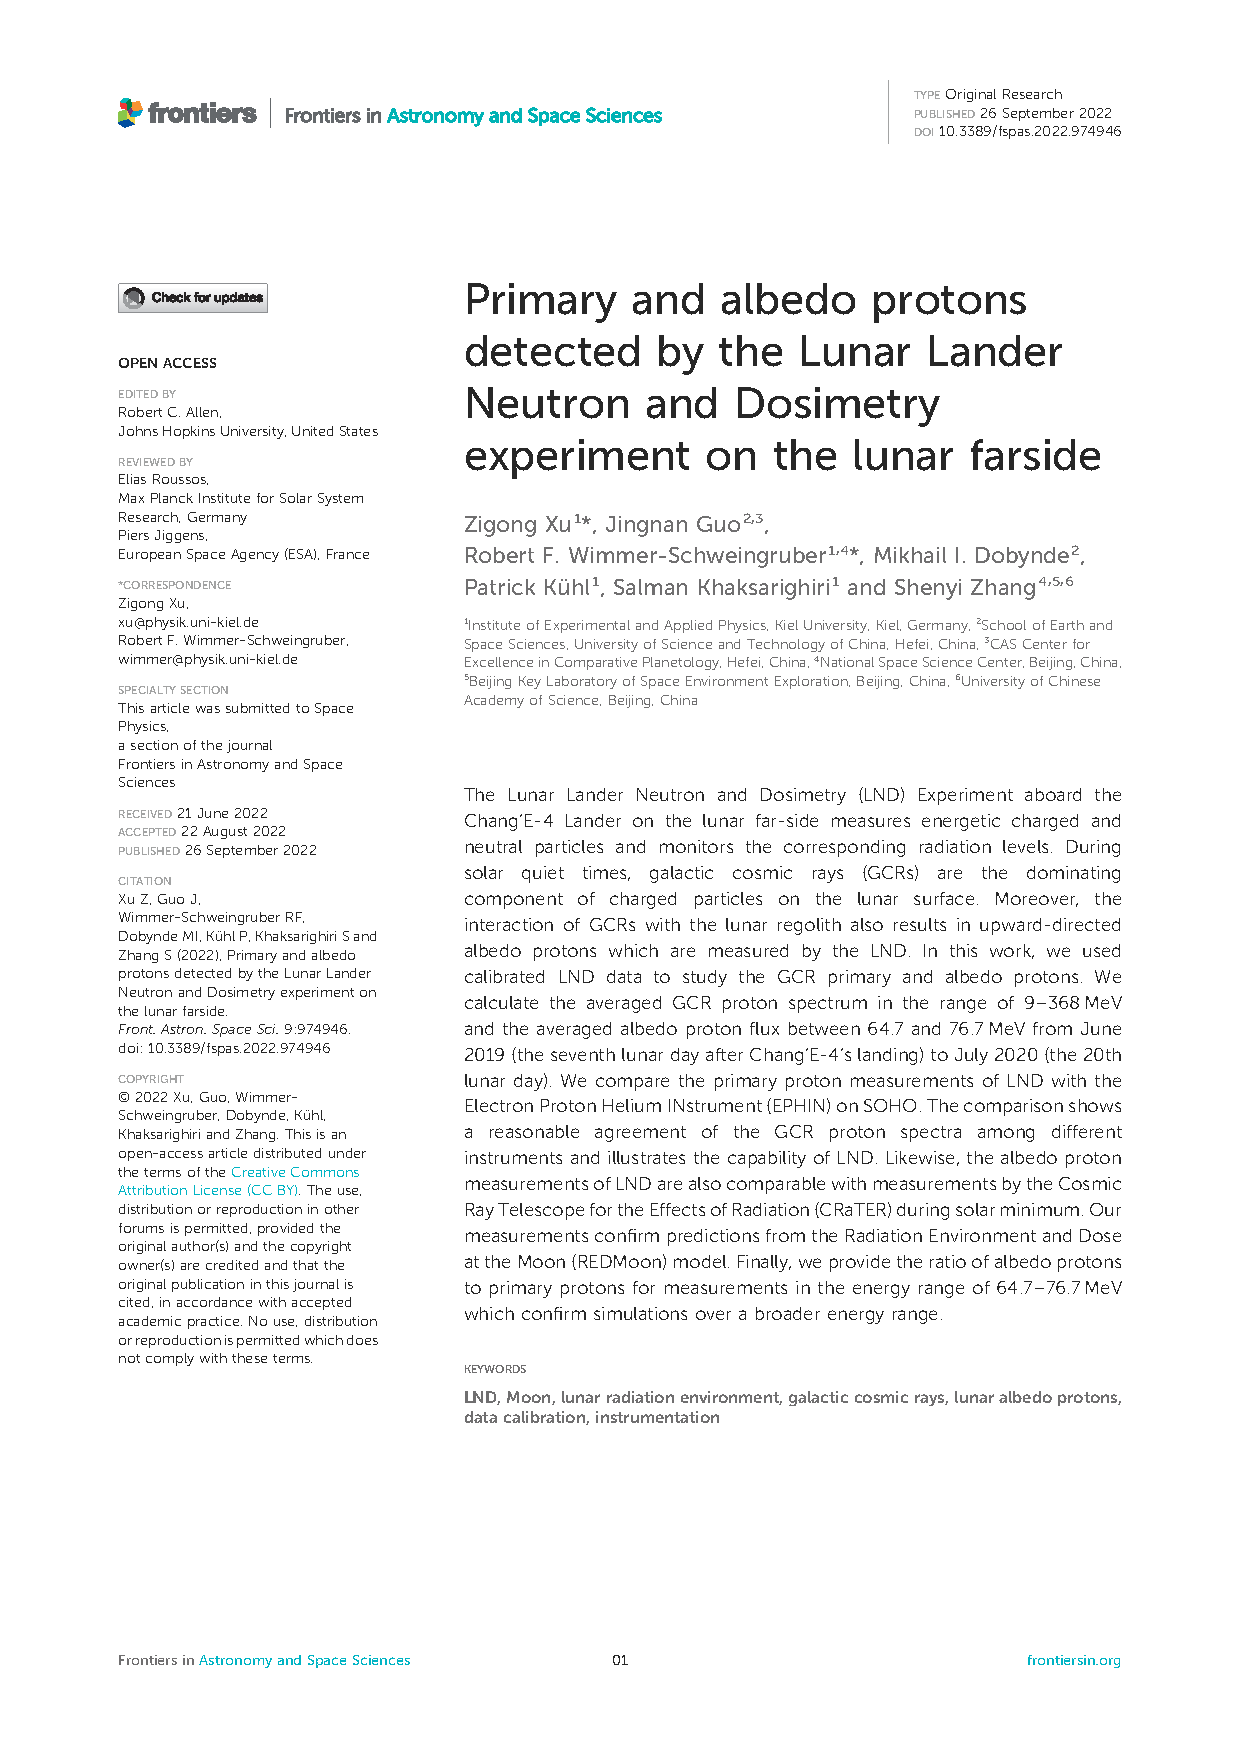
\includepdf[pages={1-3}, link, linkname=paper_xu2022, scale=.9, pagecommand={\refstepcounter{includepdfpageFrontierTwentyTwo}\label{paper_xu2022.\theincludepdfpageFrontierTwentyTwo}}]{publications/Xu_et_al_2022_Frontier.pdf}
%
\addtocounter{subsubsection}{1} 
\phantomsection
\addcontentsline{toc}{subsubsection}{\arabic{chapter}.\arabic{section}.\arabic{subsection}.\arabic{subsubsection} Preparation of LND data}
\includepdf[pages={4-8}, link, linkname=paper_xu2022, scale=.9, pagecommand={\refstepcounter{includepdfpageFrontierTwentyTwo}\label{paper_xu2022.\theincludepdfpageFrontierTwentyTwo}}]{publications/Xu_et_al_2022_Frontier.pdf}
%
\addtocounter{subsubsection}{1} 
\phantomsection
\addcontentsline{toc}{subsubsection}{\arabic{chapter}.\arabic{section}.\arabic{subsection}.\arabic{subsubsection} Measurements and comparison with model}
\includepdf[pages={9-11}, link, linkname=paper_xu2022, scale=.9, pagecommand={\refstepcounter{includepdfpageFrontierTwentyTwo}\label{paper_xu2022.\theincludepdfpageFrontierTwentyTwo}}]{publications/Xu_et_al_2022_Frontier.pdf}
%
\addtocounter{subsubsection}{1} 
\phantomsection
\addcontentsline{toc}{subsubsection}{\arabic{chapter}.\arabic{section}.\arabic{subsection}.\arabic{subsubsection} Summary, discussion and conclusion}
\includepdf[pages={12}, link, linkname=paper_xu2022, scale=.9, pagecommand={\refstepcounter{includepdfpageFrontierTwentyTwo}\label{paper_xu2022.\theincludepdfpageFrontierTwentyTwo}}]{publications/Xu_et_al_2022_Frontier.pdf}
%
\addtocounter{subsubsection}{1} 
\phantomsection
\addcontentsline{toc}{subsubsection}{\arabic{chapter}.\arabic{section}.\arabic{subsection}.\arabic{subsubsection} References}
\includepdf[pages={13-14}, link, linkname=paper_xu2022, scale=.9, pagecommand={\refstepcounter{includepdfpageFrontierTwentyTwo}\label{paper_xu2022.\theincludepdfpageFrontierTwentyTwo}}]{publications/Xu_et_al_2022_Frontier.pdf}
%
\addtocounter{subsubsection}{1} 
\phantomsection
\addcontentsline{toc}{subsubsection}{\arabic{chapter}.\arabic{section}.\arabic{subsection}.\arabic{subsubsection} Supplement material}
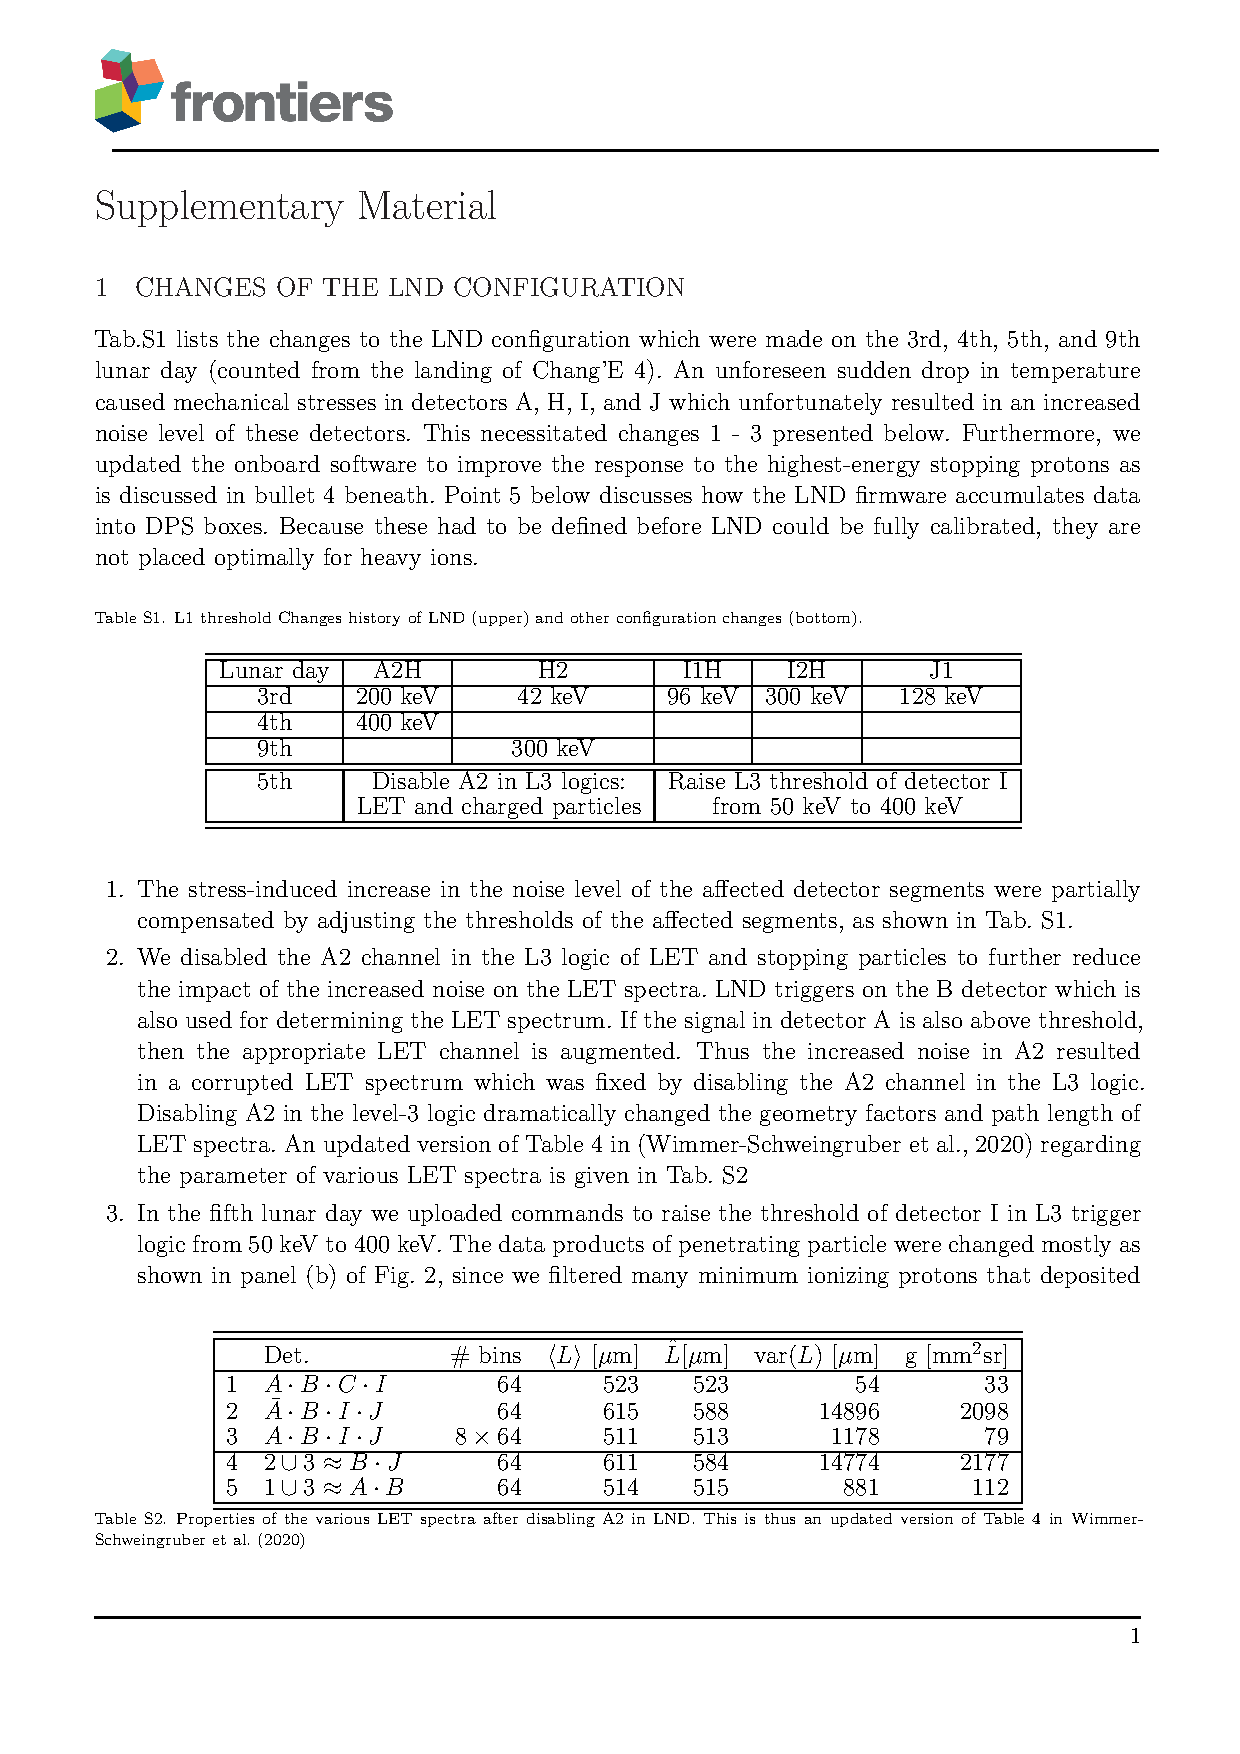
\includepdf[pages={1-3}, link, linkname=paper_xu2022, scale=.9, pagecommand={\refstepcounter{includepdfpageFrontierTwentyTwo}\label{paper_xu2022.\theincludepdfpageFrontierTwentyTwo}}]{publications/Xu_et_al_2022_frontier_appendix.pdf}